\documentclass[12pt]{report}
\usepackage[utf8]{inputenc}
\usepackage[russian]{babel}
%\usepackage[14pt]{extsizes}
\usepackage{listings}
\usepackage{graphicx}
\usepackage{amsmath,amsfonts,amssymb,amsthm,mathtools} 
\usepackage{pgfplots}
\usepackage{filecontents}
\usepackage{float}
\usepackage{indentfirst}
\usepackage{eucal}
\usepackage{enumitem}
%s\documentclass[openany]{book}
\frenchspacing

\usepackage{indentfirst} % Красная строка

\usetikzlibrary{datavisualization}
\usetikzlibrary{datavisualization.formats.functions}

\usepackage{amsmath}


% Для листинга кода:
\lstset{ %
	language=c,                 % выбор языка для подсветки (здесь это С)
	basicstyle=\small\sffamily, % размер и начертание шрифта для подсветки кода
	numbers=left,               % где поставить нумерацию строк (слева\справа)
	numberstyle=\tiny,           % размер шрифта для номеров строк
	stepnumber=1,                   % размер шага между двумя номерами строк
	numbersep=5pt,                % как далеко отстоят номера строк от подсвечиваемого кода
	showspaces=false,            % показывать или нет пробелы специальными отступами
	showstringspaces=false,      % показывать или нет пробелы в строках
	showtabs=false,             % показывать или нет табуляцию в строках
	frame=single,              % рисовать рамку вокруг кода
	tabsize=2,                 % размер табуляции по умолчанию равен 2 пробелам
	captionpos=t,              % позиция заголовка вверху [t] или внизу [b] 
	breaklines=true,           % автоматически переносить строки (да\нет)
	breakatwhitespace=false, % переносить строки только если есть пробел
	escapeinside={\#*}{*)}   % если нужно добавить комментарии в коде
}


\usepackage[left=2cm,right=2cm, top=2cm,bottom=2cm,bindingoffset=0cm]{geometry}
% Для измененных титулов глав:
\usepackage{titlesec, blindtext, color} % подключаем нужные пакеты
\definecolor{gray75}{gray}{0.75} % определяем цвет
\newcommand{\hsp}{\hspace{20pt}} % длина линии в 20pt
% titleformat определяет стиль
\titleformat{\chapter}[hang]{\Huge\bfseries}{\thechapter\hsp\textcolor{gray75}{|}\hsp}{0pt}{\Huge\bfseries}


% plot
\usepackage{pgfplots}
\usepackage{filecontents}
\usetikzlibrary{datavisualization}
\usetikzlibrary{datavisualization.formats.functions}

\begin{document}
	%\def\chaptername{} % убирает "Глава"
	\thispagestyle{empty}
	\begin{titlepage}
		\noindent \begin{minipage}{0.15\textwidth}
			
\includegraphics[width=\linewidth]{img/b_logo}
		\end{minipage}
		\noindent\begin{minipage}{0.9\textwidth}\centering
			\textbf{Министерство науки и высшего образования Российской Федерации}\\
			\textbf{Федеральное государственное бюджетное образовательное учреждение высшего образования}\\
			\textbf{~~~«Московский государственный технический университет имени Н.Э.~Баумана}\\
			\textbf{(национальный исследовательский университет)»}\\
			\textbf{(МГТУ им. Н.Э.~Баумана)}
		\end{minipage}
		
		\noindent\rule{18cm}{3pt}
		\newline\newline
		\noindent ФАКУЛЬТЕТ $\underline{\text{«Информатика и системы управления»}}$ \newline\newline
		\noindent КАФЕДРА $\underline{\text{«Программное обеспечение ЭВМ и информационные технологии»}}$\newline\newline\newline\newline\newline
		
		\begin{center}
			\noindent\begin{minipage}{1.1\textwidth}\centering
				\Large\textbf{  Отчет по лабораторной работе №4}\newline
				\textbf{по дисциплине <<Функциональное и логическое}\newline
				\textbf{~~~программирование>>}\newline\newline
			\end{minipage}
		\end{center}
		
		\noindent\textbf{Тема} $\underline{\text{Функции языка Lisp~~~~~~~~~~~}}$\newline\newline
		\noindent\textbf{Студент} $\underline{\text{Романов А.В.~~~~~~~~~~~~~~~}}$\newline\newline
		\noindent\textbf{Группа} $\underline{\text{ИУ7-63Б~~~~~~~~~~~~~~~~~~~~~~~}}$\newline\newline
		\noindent\textbf{Оценка (баллы)} $\underline{\text{~~~~~~~~~~~~~~~~~~~~~~}}$\newline\newline
		\noindent\textbf{Преподаватель} $\underline{\text{Толпинская Н.Б.}}$\newline\newline\newline
		
	\begin{center}
		\vfill
		Москва~---~\the\year
		~г.
	\end{center}
\end{titlepage}
	
	
	
\section*{Задание 1}
\subsection*{Постановка задачи}
	
Написать функцию, которая переводит температуру в системе Фаренгейта в температуру по Цельсию.
	
\subsection*{Решение}

\begin{lstlisting}[label=first,caption=Решение задания №1, language=lisp]
(defun fahrenheit-celsius (temp)
	(* (/ 5 9) (- temp 32.0)))
\end{lstlisting}

\section*{Задание №2}
\subsection*{Постановка задачи}
Что получится при вычислении каждого из выражений?

\subsection*{Решение}

\begin{lstlisting}[label=second,caption=Решение задания №2, language=lisp]
(list `cons t NIL) -> (CONS T NIL)
(eval (eval (list `cons t NIL))); The function T is undefined
(apply #`cons `(t NIL)) -> (T)
(list `eval NIL) -> (EVAL NIL)
(eval (list `cons t NIL)) -> (T)
(eval NIL) -> NIL
(eval (list `eval NIL)) -> NIL
\end{lstlisting}

\section*{Задание №3}
\subsection*{Постановка задачи}
Написать функцию, вычисляющую катет по заданной гипотенузе и другому катету прямоугольного треугольника, и составить диаграмму ее вычисления.

\subsection*{Решение}
\begin{lstlisting}[label=third,caption=Решение задания №3, language=lisp]
(defun get-cathetus (c a)
	(sqrt (- (* c c) (* a a))))
\end{lstlisting}

\section*{Задание №4}
\subsection*{Постановка задачи}
Написать функцию, вычисляющую площадь трапеции по ее основаниям и высоте, и составить диаграмму ее вычисления.

\subsection*{Решение}
\begin{lstlisting}[label=4xxd,caption=Решение задания №4, language=lisp]
(defun trapezium-area (a b h)
	(* (/ (+ a b) 2) h))
\end{lstlisting}

\section*{Контрольные вопросы}
\textbf{Вопрос 1.} Синтаксическая форма и хранение программы в памяти.

\textbf{Ответ.}
В Lisp формы представления программы и обрабатываемых ею данных одинаковы – они представлены в виде S-выражений. Программы могут обрабатывать и преобразовывать другие программы или сами себя. В памяти программа представляется в виде бинарных узлов, так как она состоит из S-выражений.\newline

\textbf{Вопрос 2.} Трактовка элементов списка. 

\textbf{Ответ.}
Если отсутствует блокировка вычислений, то первый элемент списка трактуется как имя функции, а остальные элементы – как аргументы функции.\newline

\begin{figure}[H]

	\begin{center}

		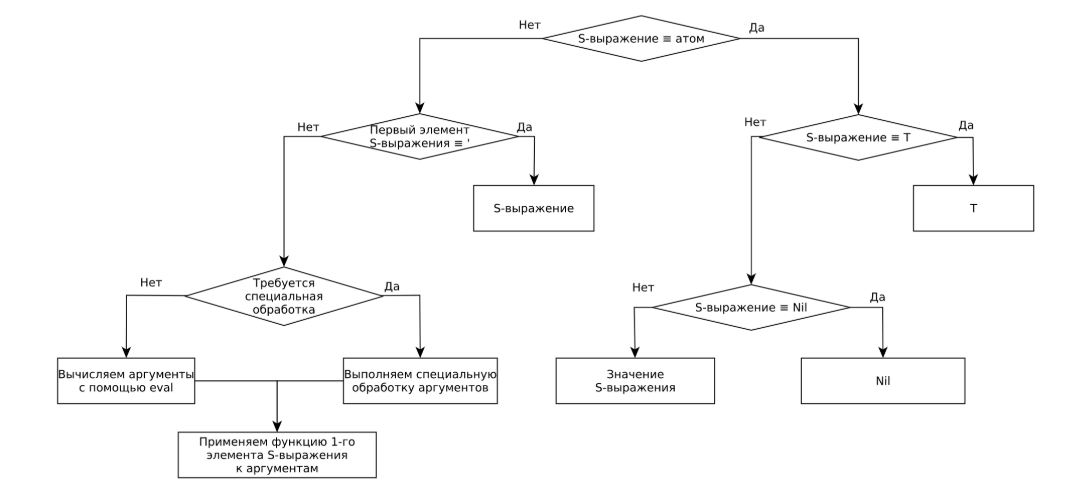
\includegraphics[scale=0.4]{img/eval.png}

	\end{center}
	\caption{Схема работы функции \textbf{eval}.}

	\label{img:eval}

\end{figure}
	
\textbf{Вопрос 3.} Порядок реализации программы.

\textbf{Ответ.}
Работа программы циклична: сначала программа ожидает ввода S-выражения, затем передает полученное S-выражение интерпретатору – функции eval, а в конце, после отработки функции eval, выводит последний полученный результат.\newline

	
\textbf{Вопрос 4.} Способы определения функции.

\textbf{Ответ.}
Функцию можно определить с помощью \textbf{defun} или \textbf{lambda.} (defun имя\_функции (список\_аргументов) тело\_функции).
	
\bibliographystyle{utf8gost705u}  % стилевой файл для оформления по ГОСТу
	
\bibliography{51-biblio}          % имя библиографической базы (bib-файла)
	
	
\end{document}
